\documentclass[output=paper]{langsci/langscibook}
\ChapterDOI{10.5281/zenodo.573779}

\author{Dan Dediu\affiliation{Max Planck Institute for Psycholinguistics, Nijmegen,
The Netherlands}}
\title{From biology to language change and diversity} 
\maketitle\begin{document}
\section{Introduction}   

Establishing \textsc{causality} (or at least, attempting to) must rank as one of the most important aims of science, but despite the widespread impression to the contrary, any cursory look at the vast literature dedicated to it or, for that matter, to the scientific literature where claims to have established, supported or refuted causal stories abound, shows that this is a very complex, multifaceted and slippery concept. Indeed, the philosophical literature abounds with proposals of what causality is and how it can be established, as well as counter-examples and counter-proposals, while there recently has been an explosion in the methodological literature mostly fueled by the seminal work of Judea Pearl (\citealt{Pearl2000}; see also Blasi \& Roberts 2017, in this volume). 

Given the complexity of this literature and the brevity of this chapter, I will use here the guide laid down by the “Causality in the Sciences” (CitS) movement\footnote{This is far from being the only proposal (or non-controversial), but I find it the best available framework for the practicing scientist with limited time and resources.} \citep{Illari2011,Illari2014} which, very helpfully, distinguishes between \textsc{scientific} and \textsc{philosophical} questions. The five scientific questions concern \textsc{inference} (what are the causal relations between \textit{X} and \textit{Y} and what is their quantitative form, what are the causes of effects, what are the effects of causes), \textsc{prediction} (how do we know and with what accuracy), \textsc{explanation} (how to causally explain, how much is explained by statistics, what level of explanation), \textsc{control} (how and when to control for confounds, the experimental setting, how to interfere with a system), and \textsc{reasoning} (how to think about causality, what concepts underlie a causal story, how to “sharpen up” causal reasoning). The five philosophical questions are \textsc{epistemological} (how do we know causal relations), \textsc{metaphysical} (what is causality, what features must causes have, what sort of entities are causes), \textsc{methodological} (how to study causality; this is related to \textsc{inference}), \textsc{semantic} (what do we mean by causality, what concept of causality is used), and \textsc{use} (what are we using causal knowledge for). Keeping these problems distinct helps not only by keeping the research questions and methods on the right track, but also avoids muddled discussions and debates where different questions are addressed (knowingly or not) by different parties, arguing at cross purposes. Moreover, there are two very important distinctions that are sometimes glossed over, namely the relation between the \textsc{population} (or type)-level and \textsc{individual} (or token)-level causes (e.g., dry climate might reduce the probability of tone but how does that relate to \ili{Berber} not having tone but \ili{Khoekhoe} having a complex tone system?), and the difference between \textsc{difference-making} (or probability-altering, e.g., correlations, associations, counterfactuals) and \textsc{mechanistic} (or production, e.g., substantive mechanisms, process, information flow) views of causality.

With these in mind, we must acknowledge first that causal explanations in linguistics (broadly speaking) are hard not only because of historical accidents that meant that important sections of our discipline were quite reluctant to use numbers, viewed variation with suspicion and felt that it must be explained away, and resisted non-linguistic factors as (partial) causes of interesting linguistic patterns, but also because language is intrinsically difficult. It spans multiple levels of organization, spatio-temporal scales and scientific disciplines, and it involves humans and their cultures. This complexity means that, ideally, claims should be supported by multiple strands of evidence possibly from different disciplines and using different methodologies, each reinforcing each other and the overall proposal, but this is unfortunately very hard to achieve in practice. Nevertheless, if we want to have a full, convincing and coherent account of why language is the way it is and how it came to be so, we must embrace these challenges and try to build causal bridges from molecules to linguistic diversity, bridges that will differ in complexity depending on the particular proposals concerned, but that share a common blueprint.

\section{From molecules to linguistic diversity}

I will briefly review two examples of such attempts at building bridges across levels and disciplines, one focusing on tone and the other on clicks. Even if either (or both) of these accounts should prove false (which in itself will be proof that the scientific methods work as they should even for such complex cases!), I hope the overarching program will be successful in advancing our understanding, methodology and way of thinking about language and its causes.

\section{Tone and genes (and climate)}
\is{tone} \is{genetics} \is{climate} \is{pitch} \is{dynamic phenomena} \is{tonogenesis}
All spoken languages use voice pitch to convey information as intonation \citep{Ladd2008intonation} but in about half of the world's languages (so-called \textsc{tone} languages; \citealt{Maddieson2013b} and the associated map at \url{http://wals.info/feature/13A}) it is also used to encode words and grammatical distinctions \citep{Yip2002}. While the distinction between languages that do and do not have tone (and the type and number of tones in the tone languages) is not clear-cut and simple to establish, a typology of tone can be usefully applied. The geographic distribution of tone languages is non-random \citep{Maddieson2013b} and tone is a dynamic phenomenon in the sense that tone can be gained (\textsc{tonogenesis}) and lost, tends to be retained in language families (i.e., it carries a genealogical signal)\is{genealogical signal}\is{language contact}\is{production}\is{perception}but can be influenced by contact with other languages too. This pattern thus requires a causal account, and there are several proposals appealing to language-internal factors (such as universal properties of speech production and perception), treating the dynamics of tone as a purely linguistic phenomenon \citep{Yip2002}.

However, this pattern might very well be also influenced by extra-linguistic factors that combine with the linguistic ones to produce a more complex, nuanced and – ultimately – interesting causal account. One such factor was suggested by Bob Ladd and myself almost a decade ago \citep{Dediu2007}, based on the idea that\textit{very weak biases} \is{biases!weak}\is{transmission!cultural}\is{computer models} \is{iterated learning}at the individual level (so weak in fact that they cannot be detected without very sensitive experimental techniques) might be amplified by the inter-generational cultural transmission of language, influencing the trajectory of language change and resulting in observable patterns of linguistic diversity \citep{Dediu2011b,Ladd2008intonation}. This mechanism has been shown to work in computer models \citep{Dediu2008,KirbyEtAl2002,Kirby2007} and iterated learning experiments with human participants \citep{Kirby2008,Smith2010}.

Our specific proposal concerned two genes involved in brain growth and development (\textit{ASPM} and \textit{Microcephalin}) for which two so-called \textsc{derived alleles} \is{derived alleles} exist whose population frequency correlate very strongly with the probability that a population speaks a tone language or not. Of course, correlations can be spurious and a major concern for correlational studies, especially using large databases, is that such meaningless correlations are bound to pop up, and proper methods to control for them are required \citep{LaddEtAl2015}. However, even after controlling for the historical relatedness and the geographic distance between the languages in our sample (within the limits of our data and the methods available), and even after comparing the relationship between tone, \textit{ASPM} and \textit{Microcephalin} with the (literally) millions of possible relationships between 26 structural features of languages and 981 genetic loci spread across the genome, we found that tone is predicted by the population frequency of these two genes much better than expected by chance.\footnote{A better control for the fact that our hypothesis was prompted by the maps of tone and the two derived alleles would be represented by testing the hypothesis on a new set of populations and languages but, unfortunately, this is still not feasible. However, our testing against the 26 features and 981 markers does support the strength of the hypothesized association within the limits of available data.}

\is{biases!weak} \is{perception} \is{production} \is{tone} \is{transmission!cultural}
We then tried to spell out an as-detailed-as-possible proposal for how these two genes could affect tone: at the individual level, these genes influence (during development and/or afterwards) a weak bias affecting the acquisition, perception, production and/or processing of tone, a bias that differs among individuals carrying different genotypes at these two genes. Therefore, populations with varying frequencies of these different individuals experience different types and level of this bias, an inter-population difference that is amplified by the inter-generational cultural transmission of language (in a feed-back loop) resulting in different trajectories of language change and, finally, a patterned distribution of tone \citep{Dediu2011b,Dediu2007}\footnote{Another feed-back loop that we did not discuss is the logical possibility that existing patterns of linguistic diversity (such as for tone) might in turn generate pressure on our genomes resulting in adaptations for particular types of languages through some form of the Baldwin effect. However, even though this proposal has been repeatedly suggested to us, I believe that the time-scales and putative selective pressures (if any) involved make such a scenario quite improbable.}. 

\largerpage
The evidence so far for this causal account is patchy and consists (besides the correlation between population genetics and tone distribution in our original paper) of computer models\is{computer models} \is{derived alleles}showing that such biases can work and might result in observable geographic patterns \citep[e.g.,][]{Dediu2008,Dediu2009} and \citegen{Wong2012} finding that \textit{ASPM} is associated with lexical tone perception within individuals.\footnote{This study, while very interesting and using two different measures of lexical tone, suffers from a small sample size and, apparently problematic for us, while finding an effect where we predicted it should be, the effect is seemingly in the opposite direction (but see the caveats in \citegen{Wong2012} and the fact that their measure is probably a measure of intonation and not of lexical tone, making their result match perfectly with our prediction; see \citealt{Caldwell-Harris2015}).} However, it is still unclear, at the molecular, cellular and neuro-cognitive levels, what exactly these derived alleles might do to influence a bias affecting tone, and what precisely this bias looks like (and not for want of testing hypotheses, ranging from the missing fundamental \citealt{Ladd2013}, artificial tone language learning \citealt{Asaridou2015} and syllable segmentation using tone \citealt{Caldwell-Harris2015}), but, so far, the decisive evidence one way or the other is still lacking (such as a well-designed sufficiently powered inter-individual genetic association study), making this hypothesis still open to empirical testing.

\is{tone}
A new exciting twist, making this complex causal story even more interesting, is represented by the suggestion that climate \is{climate} influences the patterning of tone \citep{Everett2015} in the sense that air dryness biases against the retention of tone. Moreover, Collins (2017, in this volume) suggests that tone simply reflects past demographic movements as captured by mitochondrial haplotypes, which raises interesting questions about the genealogical stability of tone \citep{Dediu2011a}. Nevertheless, the really intriguing prospect is that all these factors (and many more) play a role in shaping the temporal dynamics and geographic patterning of tone, weaving a complex and fascinating causal story involving multiple different factors (phonetics, genetics, climate, demography) acting at different scales and levels.

\section{Why are clicks so rare?}
\is{clicks} \is{affective meanings} \is{borrowing}
The production of clicks involves the rarefaction of air within an enclosed space in the oral cavity requiring thus no airstream from the lungs. While many languages use clicks \textit{paralinguistically} to convey affective meanings (such as irritation and disappointment), to express negation, or to interact with animals (see \citealt{Gil2013}), there are very few languages \citep[10 as counted by][]{Maddieson2013a}, geographically restricted to southern and eastern Africa (\citealt{Maddieson2013a} and associated map at \url{http://wals.info/feature/19A}), that incorporate clicks in their phonological inventory. Phonological inventories with clicks are primarily found in the “\ili{Khoisan} languages”, a set of language families (e.g., Khoe-Kwadi, \ili{Tu} and \ili{Kxa}\footnote{I use here the language families as given by the WALS \citep{DryerEtAl2013} given that I also refer to WALS feature descriptions and maps.}) and isolates (e.g, \ili{Hadza} and \ili{Sandawe}) but they have also been borrowed in some \ili{Bantu} languages (such as \ili{Zulu} and \ili{Xhosa}) and the \ili{Cushitic} language \ili{Dahalo}. The present-day fragmented range of the click languages and the known recent \ili{Bantu} expansion suggest that click languages might have had a much more extensive range in sub-Saharan Africa. \is{clicks}

This rarity and geographic clustering (notwithstanding the putative earlier extended range), combined with their prevalence as paralinguistic sounds and the fact that they can be borrowed \is{borrowing} into other languages, raises some intriguing questions. Of course, their restricted distribution can simply be a statistical fluctuation expected to obtain when enough features are considered, even in the case where there is a bias against clicks due to properties related to their acoustics, perception or production that universally disfavor them. \is{acoustics} \is{perception} \is{production} \is{clicks}

Alternatively \citep{MoisikEtAl2015}, it has been suggested that their particular geographic range is explained by the relaxation of a bias against their production due to the anatomy of the hard palate in the click-language speakers: more precisely, \citeauthor{Traill1985} (\citeyear{Traill1985}; see also \citealt{Traunmüller2003}) observed that of his five \ili{ǃXóõ} (\ili{Tu} family) speakers, four do not have an alveolar ridge (see tracings in \citealt{Traill1985} and \citealt{MoisikEtAl2015} for a comparison with a palate featuring a prominent alveolar ridge); this pattern seems to hold for much larger and comprehensive samples \citep[reviewed in][]{MoisikEtAl2015}. The suggestion was that somehow, the lack of an alveolar ridge helps in producing lingual clicks, weakening the bias against clicks in the populations with a high incidence of palates without an alveolar ridge. \is{clicks}

Scott Moisik \citep{MoisikEtAl2015} has refined this proposal by suggesting that the shape of the alveolar ridge impacts clicks production because a smooth hard palate requires less effort for the tongue to form the anterior contact, and also allows a better change in the cavity's volume during click release. He tested these hypotheses by building a realistic bio-mechanical model of (dental) click production with ArtiSynth (\href{http://www.artisynth.org/}{{www.artisynth.org}}; \citealt{Lloyd2012}) in which different shapes of the alveolar ridge were simulated. He found that when there is a large alveolar ridge more muscle effort is required and the volume change was negatively impacted, suggesting that indeed, within the limits of this initial simulation,\footnote{Currently, he is exploring ways to improve this simulation and to also include estimates of the acoustic effects of hard palate shape.} a hard palate without an alveolar ridge favors the production of (dental) clicks. \is{biomechanical modelling} \is{clicks}

Assuming these preliminary results will be supported by later refinements in the simulation, are they sufficient to support the suggested conjecture? What sort of empirical data should we attempt to collect and what type of tests should we conduct? Finally, what really is the causal structure of such claims?

\section{The causal anatomy of language}
\is{genetics} \is{biases!weak} \is{cultural evolution}
The two examples above are, in fact, special cases of a general framework that attempts to causally link biology\footnote{This framework can be easily adapted for other extra-linguistic factors such as climate (see, for example, \citealt{Everett2015}, or \citealt{LaddEtAl2015}).} and language, a framework that is the foundation of the Genetic Biases in Language and Speech (G[ɜ]bils) project funded by the Netherlands Organisation for Scientific Research (NWO) and hosted at the Max Planck Institute for Psycholinguistics in Nijmegen. The idea is that an individual's genotype (in interaction with its environment), during and after development, produces and maintains a vocal tract\footnote{and ears, and a brain, and hands, etc., but here we are focusing on vocal tracts for reasons to do with the tractability of the problem space, the availability of reliable methods of measurement and the relatively well understood principles of bio-mechanics and acoustics.} whose structure affects the individual's speech and might result in (very weak) biases in speech production, which might be expressed and amplified in populations of such biased individuals through cultural evolution, finally affecting the large-scale observable patterns of language (see \figref{fig:dediu:1}).

\begin{figure}
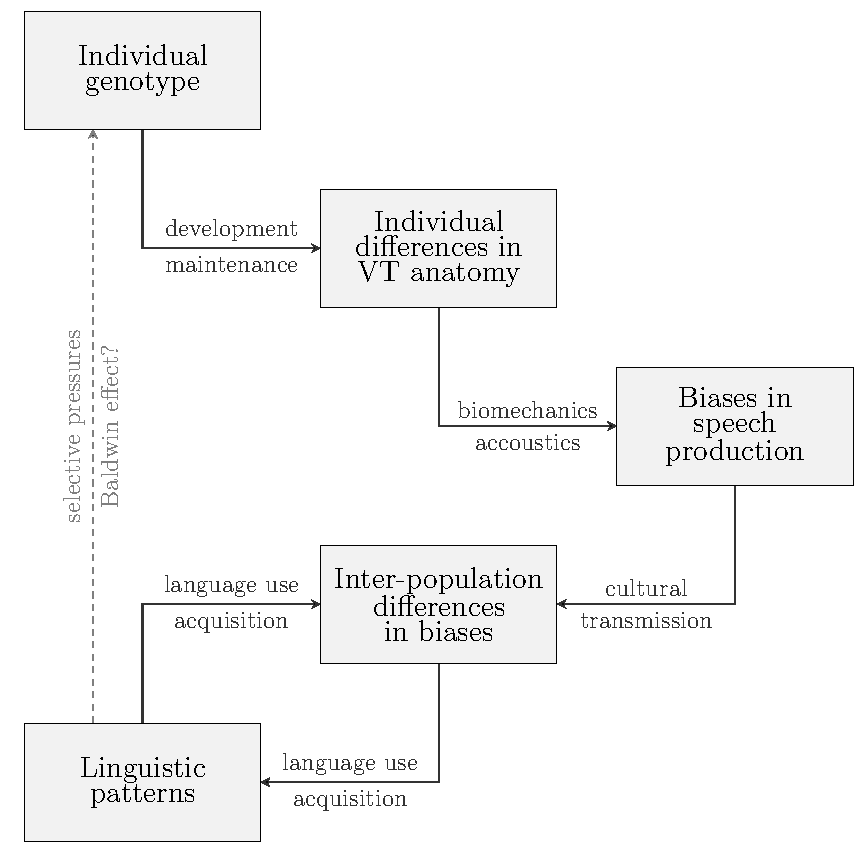
\includegraphics[width=\textwidth]{figures/dediu_flowchart.pdf}
\caption{The general causal framework connecting the molecular bases of inter-individual variation in vocal tract anatomy to language change and patterns of linguistic diversity. The boxes and links are discussed in the text (except for the feedback from linguistic patterns to the genome mediated from something like the Baldwin effect; this is a separate issue not covered in this chapter). This framework can easily be extended to also include auditory perception (see \citealt{Butcher2006} for an intriguing proposal involving Chronic Otitis Media in Australia) and cognitive processing (as forcefully argued by \citealt{Christiansen2008}; see also Christiansen 2017, this volume and Culbertson 2017, this volume).  }
\label{fig:dediu:1}
\end{figure}
\is{inter-individual differences} \is{causual chains} \is{probabilistic models}
Several important observations are in order. First, development (and maintenance) are extremely complex dynamic processes resulting from tight interaction between the genotype and the environment, involving large and structured networks of genes with surprising evolutionary histories \citep[e.g.,][]{Carroll2011}. These processes \citep{Fitch1999} result in individual anatomies of the vocal tract structures (for example, focusing on the hard palate only, its morphogenesis requires a delicate orchestration of gene networks controlling the growth, elevation, adhesion and fusion of the palatal shelf that quite often fail to a certain degree and result in pathologies such as cleft palate; see \citealt{Bush2012,Dixon2011} for reviews), and differences between individuals in the genes involved in these processes (or in the relevant environmental factors\footnote{A fascinating case is represented by type of food consumed, with the varying amount of masticatory effort affecting the anatomy of the lower jaw explaining some of the variation between hunter-gatherer and agricultural populations \citep{Cramon-Taubadel2011}.}) result in inter-individual variation in the anatomy of their vocal tracts (a still under-researched topic but see \citealt{Praveen2011,Lammert2013,Lammert2011,You2008,Liu2012}). Establishing these causal links requires investigations of normal and pathological evolution and development, understanding the genetic bases of clinical phenotypes affecting the vocal tract (e.g., cleft lip and palate), animal and cell-based models of vocal tract development, and the transfer of these findings to the normal range of variation in humans through large-scale genetic association studies. These causal chains are long, complex, and probabilistic, both mechanistic and difference-making, and must bridge from molecular mechanisms to measurable anatomical differences but, on the bright side, they stay largely within the bio-medical sciences which ensures agreed-upon standards of what a good causal story is and how it should be supported or rejected.

Second, these inter-individual differences\is{inter-individual differences}\is{acoustics} in vocal tract anatomy might cause differences between individuals in their articulatory behavior and acoustic output \citep{Brunner2005,Brunner2009,Debruyne2002}; these relationships can be empirically measured and quantified using techniques such as MRI, intra-oral scans, X-rays or 3D digitized casts and bone structures. Based on these primary data we can build computer models\is{computer models}\is{probabilistic models}\is{compensation} to investigate the articulatory and acoustic outputs, we can conduct statistical analyses (using classical and geometric morphometrics; \citealt{Zelditch2012}) and we can correlate them with measured acoustic behavior. These causal chains are relatively short, stay within articulatory phonetics, but are highly probabilistic, involve a high degree of complexity (in the sense of chaos theory) and offer many opportunities for mediation (what phoneticians usually call “compensation”; e.g. \citealt{Brunner2006}).

\largerpage
\is{inter-population differences} \is{transmission!cultural} \is{computer models} Third, these inter-individual biases in speech production are found within populations of speakers; if there are systematic differences between populations in their make-up in what concerns these biases (i.e., the distribution\footnote{Importantly, we are not talking here only about the frequency of such biases in the population (a first approximation, easy to measure and model) but, crucially, about the biases' relation to the communicative networks present in the population.} of their types and strength), then it is possible that inter-population differences will emerge, these differences will be amplified and expressed through the cultural evolution that governs language and will result in differences between the languages spoken by those populations \citep{Levinson2013}. This feedback loop is an essential causal engine and there are many opportunities for mediation resulting from population heterogeneity and other cultural forces that affect language change \citep{Dediu2011b}. We can investigate this using computer models, experimental manipulations of cultural transmission in the lab, actual historical linguistic processes, and statistical correlations between biases and cross-linguistic variation. A possible complicating factor is that we need to straddle several disciplines including historical linguistics, typology, phonetics, phonology, cognitive neuroscience, and studies of cultural evolution, which might result in different standards for causality and fundamental disagreements; moreover we probably must stay mostly within the realm of difference-making accounts as mechanistic processes are not yet understood well enough.


% In the G[ɜ]bils project, we are approaching this framework from a variety of directions and at several levels simultaneously and, while we are still in the early stages, progress being currently made gives hopes that at least some of the components of this fascinating causal story will soon be characterized. For example, Scott Moisik and myself have designed and conducted a massive study (“ArtiVark”) using MRI and 3D intra-oral scanning in an ethnically diverse sample of almost 90 participants aimed at investigating the patterns of intra- and inter-population variation in the anatomy of vocal tract structures and their relation to the articulation of various classes of sounds such as clicks, retroflex stops and fricatives, and the control of pitch. The data will be quantified using a standardized set of landmarks and semi-landmarks and subjected to statistical analyses using classical and geometric morphometrics, but Scott Moisik and Rick Janssen will also build (acoustic, articulatory and bio-mechanical) computer models to investigate the relationship between the observed anatomical variation and phonetics. We will conduct large-scale statistical and phylogenetic analyses \citep{Dediu2011a,Dediu2013,LaddEtAl2015} of databases such as PHOIBLE (Moran, 2011; \href{http://phoible.org/}{{http://phoible.org}}) and WALS \citep{DryerEtAl2013} trying to disentangle the influence of such biases on the distribution of present-day linguistic diversity and its evolution through time. Rick Janssen is also developing an agent-based computer model where the agents have realistic models of the vocal tract and individual anatomy, whereby they can learn to control these vocal tracts using neural networks and genetic algorithms, and produce the sounds in their community's language. Such agents will form heterogeneous populations of interacting language users and learners \citep{Dediu2009,Ferdinand2009} and we will investigate the effect of anatomical VT variation on the resulting languages. Finally, we are currently part of a larger collaboration where we aim to quantify VT variation in a sample of about 3000 participants from the normal population and to conduct genetic association studies (using both candidate genes from the clinical literature and unbiased genome-wide scans) to identify the genetic foundations of normal variation in these structures.

\section{Conclusions}

Establishing convincing causal stories that link language and extra-linguistic factors is inherently difficult and complex, but we can make substantial progress if we agree to take seriously the complexity of the task, the need to talk across disciplines and methods, and to think about what solid causal accounts actually imply. There is no single golden path to causality (despite what some experimentalists might think!) and we can only progress if we take a pluralistic approach that builds upon experiments (when feasible, relevant and valid), natural experiments (when we're lucky enough to find them), advanced statistical analyses of large databases (keeping in mind good practices and the highest standards of skepticism), computer models of many kinds (built on current theories and calibrated on empirical findings), recent advances in methods such as Directed Acyclic Graphs (DAGs) and Structural Equation Modeling (SEM), and any other methods that can offer valid and reliable information concerning the problems at hand.

In the end, having such an overarching causal story connecting multiple levels, scales and disciplines will not only allow us to answer all five scientific questions of causality with increased clarity and detail with respect to language and its evolution, but more importantly, to discover new interesting questions we did not even know were possible to meaningfully ask.
 
\section*{Acknowledgements} 
I wish to thank Scott Moisik specifically for his work on clicks used here as an example, but also for his and Rick Janssen's more general contributions to the G[ɜ]bils project; Carly Jaques for invaluable help with ArtiVark; Alexandra Dima for illuminating discussions and pointers to the literature concerning causality; Nick Enfield, the participants in the “Dependencies in Language” Workshop in Ardennes, June 2014, and the organizers and participants to the “Causality in the Language Sciences” Workshop in Leipzig, April 2015, for fascinating discussions and suggestions. This work was supported by a VIDI grant from the Netherlands Organisation for Scientific Research (NWO).

\newpage 

{\sloppy
\printbibliography[heading=subbibliography,notkeyword=this]
}
\end{document} 